% !TEX root = ../thesis_main.tex



\chapter[A PDF]{A PDF For The People}
\label{appendix_forthepeople}
\label{appendix_forthepeople_old}

\section[JTW]{JTW}
Here's a master equation from JTW to describe beta decay kinematics~\cite{jtw},~\cite{jtw_coulomb}:

% !TEX root = ../thesis_main.tex



% "A PDF for the People"
\bea
\omega(\cdots) \!\!\!\! \!\!\!\! \!\!\!\! \!\!\!\! && \,\,\,\, \,\,\,\, \mathrm{d} \E \, \dOmegae \, \dOmeganu 
\,\, = \,\, \frac{\FF}{(2\pi)^5} \, \pe \Ee (E_0 - \Ee)^2 \dEe \, \dOmegae \, \dOmeganu \, \nonumber\\ 
&&	\times \,\, \xi \left[
	1 + \a \frac{\vecpe\cdot\vecpnu}{\Ee\Enu} + \bFierz \frac{\m c^2}{\Ee} 
%	&& 
    + \,\,  \calign \,\, \Talign(\vecJ) 
	\left(
		\frac{\vecpe \cdot \vecpnu}{3\Ee\Enu}
		- \frac{ (\vecpe\cdot \hatj) (\vecpnu\cdot\hatj) }{\Ee\Enu}
	\right)
	\!
	%\left(
	%	\TalignExpand
	%\right)
\right. \nonumber\\ 
&&	\left. + 
	 \frac{\vecJ}{J} \cdot
	\left(
		\A \frac{\vecpe}{\Ee} 
		+ \B \frac{\vecpnu}{\Enu} 
		+ \D \frac{\vecpe \times \vecpnu}{\Ee\Enu} 
	\right)
\right]
\label{equation:jtw_master}
\eea


where, for convenience, we have defined a nuclear alignment term,
\bea
\Talign(\vecJ) &\equiv& \TalignExpand.
\eea

Note that this master equation depends on neutrino momentum, which we cannot observe directly.  Furthermore, we cannot reconstruct neutrino momenta in our decay events either, because it would be necessary to account for the momentum of the recoiling daughter nucleus, treating the decay as a three-body problem.  From an experimental standpoint, we failed to measure the momenta of the daughters in conjunction with the ``tagged'' beta decay events with which we are primarily concerned in this thesis.  From a theoretical standpoint, JTW has intentionally neglected recoil-order terms -- meaning that the daughter nucleus is treated, for the purpose of calculating the kinetic energy distribution, as being infinitely massive, and as such it has no change in kinetic energy from the decay.  This approximation makes it a bit tricky to correctly re-formulate Eq.~(\ref{equation:jtw_master}) in terms of the momentum of the daughter instead of the momentum of the neutrino.  

Fortunately, it is possible to simplify Eq.~(\ref{equation:jtw_master}) by integrating over all possible neutrino directions, such that the result no longer depends on parameters that we do not observe.  The neutrino energy itself is not a free variable in this equation, because the energy release in the decay is fixed, and given the approximation that none of that energy is allocated to the recoiling daughter, it is very straightforward to calculate the neutrino energy for a decay event in which the beta energy is known.

%We haven't integrated out the neutrino momentum.  Neutrino energy itself is a redundant parameter, I think, because we are already using an endpoint energy and a beta energy, and we are not taking recoil-order effects into account.  Also, we treat neutrinos as massless here, which is a perfectly reasonable approximation for our purposes.  For ``convenience'', let's define a nuclear alignment term, $\Talign$, so that:


The result of performing this integration over neutrino direction is:
% !TEX root = ../thesis_main.tex



% The JTW Proto-Master
\bea
\textrm{d}^3 \Gamma
&=& 
\frac{2}{(2\pi)^4} \, \FF \, \pe \Ee (E_0 - \Ee)^2 \dEe \, \dOmegae \, \xi \nonumber\\ 
&& \times \left[
	1 + \bFierz \frac{\m c^2}{\Ee} + 
	 \A  
	\left(
		\frac{\vecJ}{J} \cdot \frac{\vecpe}{\Ee} 
	\right)
\right]
\label{equation:proto_master_jtw}
\eea

\aside{We've changed the notation of d$^3\Gamma$ from the JTW master equation, while conveniently avoiding mentioning it.}

...where 
\bea
\xi = G_v^2 \, \cos\theta_C \, f_1(E).
\eea


\section[Holstein]{Holstein}
This one is harder.  But here, we've already integrated over neutrino momentum at least.  That's something.  Here's Holstein's Eq.~(52):


% !TEX root = ../thesis_main.tex



% "A PDF for the People"
\bea
\mathrm{d}^3 \Gamma &=& 2  G_v^2 \cos^2\theta_c \frac{\FF}{(2\pi)^4} \, \pe \Ee (E_0 - \Ee)^2 \dEe \, \dOmegae 
\nonumber\\
&& \times
\left\{
	F_0(\E) 
	+ \Lambda_1 F_1(\E) \hatn \cdot \frac{\vecpe}{\Ee}
	+ \Lambda_2 F_2(\E) \left[ \left( \nhat \cdot \frac{\vecpe}{\Ee} \right)^2 - \frac{1}{3}\frac{\pe^2}{\Ee^2} \right]
	\right. \nonumber\\ && \left.
	+ \Lambda_3 F_3(\E) 
		\left[ 
			\left( \hatn \cdot \frac{\vecpe}{\Ee} \right)^3
			- \frac{3}{5}\frac{\pe^2}{\Ee^2}\hatn \cdot \frac{\vecpe}{\Ee}
		\right]
\right\}
\label{equation:holstein52}
\eea



Let's define some of that notation!
Firstly, 
\bea
\textrm{Holstein's \,} \hatn &=& \textrm{JTW's \,} \hatj,
\label{eq:nequalsj}
\eea
and the 
$\Lambda_i$ are given by Holstein's Eq.~(48):
\bea
    \Lambda_1   &:=& \LambdaOne   
    \label{eq:lambda1} \\
    \Lambda_2   &:=& \LambdaTwo 
    \label{eq:lambda2} \\
    \Lambda_3   &:=& \LambdaThree .
    \label{eq:lambda3}
\eea

\aside{Note:  It's not the case that $ | \vecJ | == J $.  It's actually super fucking infuriating notation. }

We immediately see that Holstein's $\Lambda_1$ is closely related to JTW's $\frac{\vecJ}{J}$, and a bit later after John points it out to us, we see that Holstein's $\Lambda_2$ is closely related to JTW's $\Talign$.  JTW doesn't have any equivalent to $\Lambda_3$.  In particular, we find:
\bea
\Lambda_1 \hatj &=& \LambdaOne \hatj \;\; = \;\; \frac{\vecJ}{J}  \\
%\Lambda_2 \frac{(J+1)}{(2J-1)} &=& \Talign
\Lambda_2 &=& \Talign \frac{(2J-1)}{(J+1)}.
\eea
Now we'll have to deal with expanding the $F_i(\Ee)$.  %Note that these are very different from the $F_i(\Ee, u, v, s)$, and also different from the $f_i(\Ee)$.  
Holstein makes a goddamn mess of this, so here we go!  From Holstein's Eq.~(B10):
\bea
F_i(\Ee) &=& H_i(\Ee, J, J^\prime, 0).
\eea
%and from Holstein's Eq.~(B9), we see that 
%\bea
%f_i(\Ee) &=& F_i(\Ee, J, J^\prime, 0)
%\eea
From Holstein's many Eqs.~(B7), we see that the $H_i(\Ee, u, v, s)$ can be written in terms of the functions $F_i(\Ee, u, v, s)$, which we carefully note \emph{are not the same} as the functions $F_i(\Ee)$.  We further see, from Holstein's Eq.~(B9) that a further set of functions, $f_i(\Ee)$ are defined in terms of the $F_i(\Ee, u, v, s)$.  In particular, Holstein's Eq.~(B9) states that
\bea
f_i(\Ee) &=& F_i(\Ee, J, J^\prime, 0).
\eea
Then, if we combine (some parts of) Holstein's Eqs.~(B7) with (B9) and (B10)

\begin{align}
F_0(\Ee) & \;\;=\;\; H_0(\Ee, J, J^\prime, 0) \;\;=\;\; F_1(\Ee, J, J^\prime, 0) 
	\!\!\!\! \!\! \!\! 
	& =\;\; & f_1(\Ee) 
	\\
F_1(\Ee) & \;\;=\;\; H_1(\Ee, J, J^\prime, 0) \;\;=\;\; F_4(\Ee, J, J^\prime, 0) \,\,+ \frac{1}{3}F_7(\Ee, J, J^\prime, 0) 
	\!\!\!\! \!\! \!\! 
	& =\;\; & f_4(\Ee) \,\,+ \frac{1}{3}f_7(\Ee) 
	\\
F_2(\Ee) & \;\;=\;\; H_2(\Ee, J, J^\prime, 0) \;\;=\;\; F_{10}(\Ee, J, J^\prime, 0) + \frac{1}{2}F_{13}(\Ee, J, J^\prime, 0) 
	\!\!\!\! \!\! \!\! 
	& =\;\; & f_{10}(\Ee) + \frac{1}{3}f_{13}(\Ee) 
	\\
F_3(\Ee) & \;\;=\;\; H_3(\Ee, J, J^\prime, 0) \;\;=\;\; F_{18}(\Ee, J, J^\prime, 0) 
	\!\!\!\! \!\! \!\! 
	& =\;\; & f_{18}(\Ee) .
\end{align}
So that's fun.  Note that the $f_i(\Ee)$ are what goes into the polarized decay spectrum when the neutrino (ie, the recoil) is also observed.  It's a more complicated spectrum that way.  For this spectrum in which the neutrino has already been integrated over, we can just look up the $H_i(\Ee, J, J^\prime, 0) = H_i(\Ee, u, v, s)$ spectral functions, and leave it at that.

So let's do this thing!
\begin{multline}
F_0(\Ee) = 
\left| a_1 \right|^2 
+ 2 Re\left[ a_1^* a_2 \right] \frac{1}{3 M^2} 
\left[  
	\m^2 + 4 \Ee E_0 + 2 \frac{\me^2}{\Ee}E_0 - 4\Ee^2
\right]
\\
+ \left| c_1 \right|^2
+ 2 Re\left[ c_1^* c_2\right] \frac{1}{9 M^2} 
\left[
	11 \me^2 + 20 \Ee E_0 
	- 2\frac{\me^2}{\Ee}E_0
	- 20\Ee^2
\right]
- 2 \frac{E_0}{3M} Re\left[ c_1^*(c_1 + d \pm b)\right]
\\
+ \frac{2\Ee}{3M} 
\left( 
	3 \left| a_1 \right|^2 + Re \left[ c_1^*(5c_1 \pm 2 b) \right]
\right)
- \frac{\me^2}{3 M \Ee} 
Re \left[ 
	-3 a_1^*e + c_1^*\left(2c_1 + d \pm 2b - h\frac{E_0 - \Ee}{2M} \right)
\right]
\end{multline}
% comment comment comment...
\begin{multline}
F_1(\Ee) = 
\deltauv \left( \frac{u}{\!u+1\!} \right)^{\!\!1/2} \!\!
\left\{
	2 Re\left[ 
		a_1^*\left(\! c_1 - \frac{E_0}{3M}(c_1 + d \pm b) + \frac{\Ee}{3M}( 7 c_1 \pm b + d )\! \right)
	\right]
	\right.\\\left.
	+
	2 Re\left[
		a_1^* c_2 + c_1^* a_2
	\right] \!
	\left(
		\frac{4 \E(E_0 - \E) + 3 \me^2}{3M^2}
	\right) \!
\right\}
\\
\mp \frac{ (-1)^s \gammauv}{u+1} 
Re \left[
	c_1^*\left(
		c_1 + 2 c_2 \left(\frac{8\Ee(E_0-\Ee)+3\me^2}{3M^2}\right)
		- \frac{2 E_0}{3 M} (c_1 + d \pm b) 
		+ \frac{\Ee}{3M} (11 c_1 - d \pm 5 b)
	\right)
\right]
\\
+ 
\frac{\lambdauv}{u+1}
Re \left[
	c_1^* \left(
		- f \left(\frac{5\Ee}{M}\right)
		+ g \left( \frac{3}{2} \right)^{\!\!1/2} \!
		\left(
			\frac{E_0^2 - 11 E_0 \Ee + 6 \me^2 + 4\Ee^2 }{6M^2}
		\right)
		\pm 3 j_2 
		\left(
			\frac{8 \Ee^2 - 5E_0 \Ee - 3 \me^2}{6M^2}
		\right)
	\right)
\right]
\end{multline}
%
\begin{multline}
F_2(\Ee) = 
\thetauv \frac{\Ee}{2M} 
Re\left[
	c_1^*\left(
		c_1 + c_2 \frac{8(E_0-\Ee)}{3M}
		-d \pm b
	\right)
\right]
\\
- \deltauv \frac{\Ee}{M} 
\left[ \frac{u(u+1)}{(2u-1)(2u+3)} \right]^{1/2} \!
Re \left[
	a_1^*\left( 
		\left( \frac{3}{2} \right)^{\!1/2}\! f
		+ g \frac{\Ee+2E_0}{4M} 
		\pm \left( \frac{3}{2} \right)^{\!1/2}\! j_2 \frac{E_0-\E}{2M}
	\right)
\right]
\\
+ (-1)^s \kappauv \frac{\E}{2M}
Re \left[
	c_1^* \left(
		\pm 3 f 
		\pm \left( \frac{3}{2} \right)^{\!1/2}\! g \frac{E_0-\Ee}{M}
		+ 3 j_2 \frac{E_0-2\Ee}{2M}
	\right)
\right]
+ \epsilonuv Re\left[ c_1^* j_3 \right]
\left( 
	\frac{21 \E^2}{8 M^2}
\right)
\end{multline}
%
\begin{multline}
F_3(\Ee) = 
- \deltauv (3 u^2 + 3 u -1)
\left[
	\frac{u}{(u-1)(u+1)(u+2)(2u-1)(2u+3)}
\right]^{1/2}\!
Re \left[
	a_1^* j_3
\right]
\left( 
	\frac{\Ee^2 \sqrt{15} }{4M^2}
\right)
\\
+ 
\frac{\rhouv}{u+1} 
Re\left[
	c_1^*(g\sqrt{3} + j_2\sqrt{2})
	\left(
		\frac{5 \Ee^2}{4 M^2}
	\right)
\right]
\pm
\frac{(-1)^s \sigmauv }{u+1} 
Re \left[ c_1^*j_3 \right] 
\left( 
	\frac{5\Ee^2}{2 M^2}
\right)
\end{multline}
...Phew!  I typed all of that out just so that I can have a record of what's going on here, but actually, the very first thing I want to do is make some simplifications here.  If we evaluate Holstein's Eqs.~(B8), which I will absolutely not type out here, for the case $u=v=J=J^\prime=3/2$, we find the following values:
\begin{align}
\deltauv     &= 1 
& \thetauv   &= 1 
& \rhouv     &= \frac{-41}{40}
	\nonumber\\
\gammauv     &= 1 
& \kappauv   &=\frac{1}{2\sqrt{2}} % \;\; ! \!=\;\; \frac{3}{\sqrt{2}}
& \sigmauv   &= \frac{-41}{4\sqrt{35}}
	\nonumber\\
\lambdauv    &= \frac{-\sqrt{2} }{5} % 2\sqrt{3} 
& \epsilonuv &= \frac{-1}{2\sqrt{5}}
& \phiuv     &= 0 % \frac{1}{32} \left(\frac{3}{5}\right)^{\!1/2}.
	\nonumber\\
%
\end{align}
Furthermore, in our calculations here, we will be considering only the $\beta^+$ decay modes, and therefore we take the \emph{lower} sign when the option arises.  We also will use $s=0$, so that $(-1)^s = +1$.



% %%%%%%%%%%%%%%%%%%%%%%%%%%%%%% 
% \subsubsection[Algebra]{Algebra}
% Oookay.  Here's some stuff I'll want to keep track of now, but will also want to not have cluttering my documents later.
% \begin{align}
% \deltauv \left( \frac{u}{u+1} \right)^{\!\!1/2} \;\;&=\;\; \left( \frac{3}{5} \right)^{1/2}
% \\
% \mp \frac{ (-1)^s \gammauv}{u+1} \;\;&=\;\; \frac{2}{5}
% \\
% \frac{\lambdauv}{u+1} \;\;&=\;\; \frac{4 \sqrt{3}}{5}
% \\
% - \deltauv \left[ \frac{u(u+1)}{(2u-1)(2u+3)} \right]^{1/2}  \;\;&=\;\;  \frac{-\sqrt{5}}{4}
% \\
% %(-1)^s \kappauv \;\;&=\;\; \frac{3}{\sqrt{2}}  % I math-ed this wrong before.  I think.
% (-1)^s \kappauv \;\;&=\;\; \frac{1}{2\sqrt{2}}
% \\
% \frac{21}{8} \epsilonuv \;\;&=\;\; \frac{-21}{16 \sqrt{35}} %\;\;=\;\;
% \\
% \!\!\!\! \!\!\!
% - \deltauv (3 u^2 + 3 u -1)
% \left[
% 	\frac{u}{(u-1)(u+1)(u+2)(2u-1)(2u+3)}
% \right]^{1/2}\!
% \left(
% 	\frac{\sqrt{15}}{4}
% \right)
% \;\;&=\;\; \frac{-41 \sqrt{3}}{16 \sqrt{7}}
% \\
% \frac{\rhouv}{u+1}\left( \frac{5}{4} \right) \;\;&=\;\; \frac{41}{80}
% \\
% \pm
% \frac{(-1)^s \sigmauv }{u+1} \left( \frac{5}{2} \right) \;\;&=\;\; \frac{-41}{4\sqrt{35}}
% \end{align}
% %%%%%%%%%%%% Probably check the math on all of these over again.
% Note:  I calculated $\kappa_{u,v}$ wrong before.  Probably.  Unclear about the order of operations in really old papers.
%
% \subsubsection[More Algebra]{More Algebra}
% So here are some simplifications, using those expressions we just calculated in the stupid section above.
% %
% \begin{multline}
% F_0(\Ee) =
%   \left| a_1 \right|^2
% + \left( \!
% 	\frac{2\Ee}{M}
% \! \right)
% \left| a_1 \right|^2
% + \left| c_1 \right|^2
% + \left( \!
% 	\frac{- 2 E_0 + 10\Ee - 2\me^2/\Ee}{3M}
% \! \right)
% \left| c_1 \right|^2
% \\
% %
% + \frac{\me^2}{3 M \Ee}
% \left(
% 	3 Re\left[a_1^*e\right] - Re\left[c_1^*d\right] + 2 Re\left[c_1^*b\right]
% \right)
% + \frac{-4\Ee}{3M} Re \left[c_1^* b \right]
% + \frac{- 2 E_0}{3M} \left( Re\left[c_1^* d\right] - Re\left[c_1^* b \right] \vphantom{2_2^2} \right)
% \\
% + \frac{2}{3 M^2}
% \left(
% 	\m^2 + 4 \Ee E_0 + 2 \me^2\frac{E_0}{\Ee} - 4\Ee^2
% \right)
% Re\left[ a_1^* a_2 \right]
% \\
% + \frac{2}{9 M^2}
% \left(
% 	11 \me^2 + 20 \Ee E_0
% 	- 2\me^2\frac{E_0}{\Ee}
% 	- 20\Ee^2
% \right)
% Re\left[ c_1^* c_2\right]
% +
% \frac{\me^2}{6 M^2} \left(\frac{E_0 - \Ee}{\Ee} \right) Re\left[c_1^*h\right]
% %%%%%%% simplified enough for now.  continue it later.
% \end{multline}
% So that one's looking pretty good.  I can probably simplify it further later.
% %
% \begin{multline}
% F_1(\Ee) =
% \frac{2\sqrt{3}}{\sqrt{5}} Re \left[ a_1^*c_1 \right]
% + \frac{2}{5} \left| c_1 \right|^2
% %\\
% +
% \frac{2}{\sqrt{15}} \left( \frac{7\Ee -E_0}{M} \right)
% 	Re \left[ a_1^*c_1 \right]
% +
% \frac{2}{15}
% \left( \frac{11 \E- 2 E_0}{M} \right)
% 	\left| c_1 \right|^2
% \\
% +
% \frac{2}{\sqrt{15}} \left( \frac{E_0 - \Ee}{M} \right)
% 	Re \left[ a_1^*b \right]
% +
% \frac{2}{\sqrt{15}} \left( \frac{\Ee - E_0}{M} \right)
% 	Re \left[ a_1^*d \right]
% \\
% +
% \frac{2}{15}
% \left( \frac{2 E_0 - 5 \E}{M} \right)
% 	Re \left[c_1^*b \right]
% +
% \frac{2}{15}
% \left( \frac{-2 E_0 - \Ee }{M} \right)
% 	Re \left[c_1^*d \right]
% \\
% -
% \frac{20\sqrt{3}}{5} \left(\frac{\Ee}{M}\right)
% 	Re \left[ c_1^* f \right]
% \\
% +
% \frac{2}{\sqrt{15}} \left( \frac{4 \E(E_0 - \E) + 3 \me}{M^2} \right) \!
% 	Re\left[ a_1^* c_2 + c_1^* a_2 \right]
% +
% \frac{4}{15} \left(\frac{8\Ee(E_0-\Ee)+3\me}{M^2}\right)
% 	Re \left[ c_1^*c_2 \right]
% \\
% +
% \left(\frac{12}{30 \sqrt{2} }\right) \left( \frac{E_0^2 - 11 E_0 \Ee + 6 \me^2 + 4\Ee^2 }{M^2} \right)
% 	Re \left[ c_1^* g \right]
% +
% \left( \frac{-12\sqrt{3}}{30}\right) \left( \frac{8 \Ee^2 - 5E_0 \Ee - 3 \me^2}{M^2} \right)
% 	Re \left[c_1^* j_2 \right]
% \end{multline}
% $F_1(\Ee)$ is definitely looking better than it was before.  Onwards!
% %
% \begin{multline}
% F_2(\Ee) =
% \left( \frac{\Ee}{M} \right)
% \left[
% 	\frac{1}{2} \left| c_1 \right|^2
% 	- \frac{1}{2} Re\left[ c_1^*d \right]
% 	- \frac{1}{2} Re\left[ c_1^* b \right]
% 	+
% 	\frac{-\sqrt{15}}{4\sqrt{2}}
% 	Re \left[ a_1^* f \right]
% 	+
% 	\frac{-3}{4\sqrt{2}}
% 		Re \left[ c_1^* f \right]
% \right]
% \\
% +
% \frac{1}{M^2}
% \left\{
% 	\frac{4}{3} \left[ \Ee(E_0-\Ee) \right] Re\left[ c_1^*c_2 \right]
% 	+
% 	\frac{-\sqrt{5}}{16} \left[ \Ee(\Ee+2E_0) \right] Re \left[ a_1^* g \right]
% 	+
% 	\frac{\sqrt{15}}{8\sqrt{2}} \left[ \Ee(E_0-\E) \right] Re \left[ a_1^* j_2 \right]
% \right.
% \\
% \left.
% 	+
% 	\frac{-\sqrt{3}}{8} \left[ \Ee(E_0-\Ee) \right] Re \left[ c_1^* g \right]
% 	+
% 	\frac{3}{8\sqrt{2}}\left[ \Ee(E_0-2\Ee) \right] Re \left[ c_1^* j_2 \right]
% 	+
% 	\frac{-21}{16\sqrt{35}} \left( \E^2 \right) Re \left[ c_1^* j_3 \right]
% \right\}
% \end{multline}
% %
% And that's good enough for now for $F_2(\Ee)$, even though it's not really very good.
% \bea
% F_3(\Ee) &=&
% \left( \frac{\Ee^2}{M^2} \right)
% \left[
% \frac{-41\sqrt{3}}{16\sqrt{7}}
% 	Re \left[ a_1^* j_3 \right]
% +
% \frac{41\sqrt{3}}{80}
% Re\left[
% 	c_1^* g
% \right]
% 	+
% \frac{41\sqrt{2}}{80}
% Re\left[
% 	c_1^* j_2
% \right]
% + \frac{-41}{4\sqrt{35}}
% 	Re \left[ c_1^*j_3 \right]
% \right]
% \eea
% To be honest, $F_3(\Ee)$ came out a lot cleaner than I was expecting.  That's pretty nice.
%
% %
% % \begin{multline}
% % F_2(\Ee) =
% % \frac{-9}{\sqrt{2}} Re \left[c_1^* f \right]
% % +
% % \frac{\Ee}{2M}
% % Re\left[
% % 	c_1^*c_1
% % \right]
% % +
% % \frac{8\Ee(E_0-\Ee)}{6M^2} Re\left[ c_1^*c_2 \right]
% % +
% % \frac{-\Ee}{2M}
% % Re\left[
% % 	c_1^*d + c_1^*b
% % \right]
% % \\
% % + \frac{-\sqrt{15}}{4 \sqrt{2}}
% % \left( \frac{\Ee}{M} \right)
% % 	Re \left[ a_1^*f \right]
% % +
% % \frac{-\sqrt{5}}{16}
% % \left( \frac{\Ee(\Ee+2E_0)}{M^2} \right)
% % 	Re \left[ a_1^*g \right]
% % +
% % \frac{\sqrt{15}}{8\sqrt{2}}
% % \left( \frac{\Ee(E_0-\E)}{M^2} \right)
% % 	Re \left[ a_1^*j_2 \right]
% % \\
% % + \frac{-3 \sqrt{3}}{2} \left(\frac{E_0-\Ee}{M} \right)
% % 	Re \left[ c_1^* g \right]
% % + \frac{9}{\sqrt{2}} \left( \frac{E_0-2\Ee}{2M} \right)
% % 	Re \left[ c_1^* j_2 \right]
% % +
% % \frac{-21}{16\sqrt{35}}
% % \left(
% % 	\frac{\E^2}{M^2}
% % \right)
% % Re\left[ c_1^* j_3 \right]
% % \end{multline}
% % %
% % I'll leave $F_2(\Ee)$ for now.  Onwards!
%
%
%
% Let's see what they are in the limit of infinite recoil mass!  (I think that corresponds to $M$ in the equations, but I should really double check that...)
% \bea
% F_0(\Ee) |_{M\rightarrow\infty} &=& \left| a_1 \right|^2 + \left| c_1 \right|^2 \\
% F_1(\Ee) |_{M\rightarrow\infty} &=& \frac{2\sqrt{3}}{\sqrt{5}} Re \left[ a_1^*c_1 \right]+ \frac{2}{5} \left| c_1 \right|^2 \\
% F_2(\Ee) |_{M\rightarrow\infty} &=& 0 \\ %\frac{-9}{\sqrt{2}} Re \left[c_1^* f \right] \\
% F_3(\Ee) |_{M\rightarrow\infty} &=& 0
% \eea
%
% Anyway, let's expand our Eq.~(\ref{eq:holsteinpdf}) in terms of $\Lambda_i$s and things.  Using Eqs.~(\ref{eq:nequalsj}, \ref{eq:lambda1}, \ref{eq:lambda2}, \ref{eq:lambda3}) and changing the labelling on our quantization axis to $\hatj$:
% \bea
% \d^3 \Gamma &=& 2  G_v^2 \cos^2\theta_c \frac{\FF}{(2\pi)^4} \, \pe \Ee (E_0 - \Ee)^2 \dEe \, \dOmegae
% \nonumber\\
% && \times
% \left\{
% 	F_0(\E)
% 	+
% 	\left(\! \LambdaOne \!\right)
% 	\left[ \hatj \cdot \hatp \right] \left(\! \frac{\pe}{\Ee} \!\right)
% 	F_1(\E)
% 	+
% 	\left(\! \LambdaTwo \!\right)
% 	\left[ \left( \jhat \cdot \hatp \right)^2 - \frac{1}{3} \right] \left(\! \frac{ \pe^2 }{\Ee^2} \! \right)%^2
% 	F_2(\E)
% 	\right. \nonumber\\ && \left.
% 	+
% 	\left(\! \LambdaThree \!\right)
% 	\left[
% 		\left( \hatj \cdot \hatp \right)^{3}
% 		-
% 		\frac{3}{5} \left( \hatj \cdot \hatp \right)
% 	\right]
% 	\left(\! \frac{\pe^3}{\Ee^3} \! \right)
% 	F_3(\E)
% \right\}
% \eea
%
%




\section{Comparing Notation between Holstein and JTW}
	This is a short guide to differences in notation, sign convention, and normalization.  There will be many tables here, chosen to aid in conversion between the two conventions.  In the mean time, here's a bunch of old handwritten notes on the topic, that I'll eventually have to typeset and process into something intelligible.  
	
	

\begin{figure}[htb]
	\centering
	{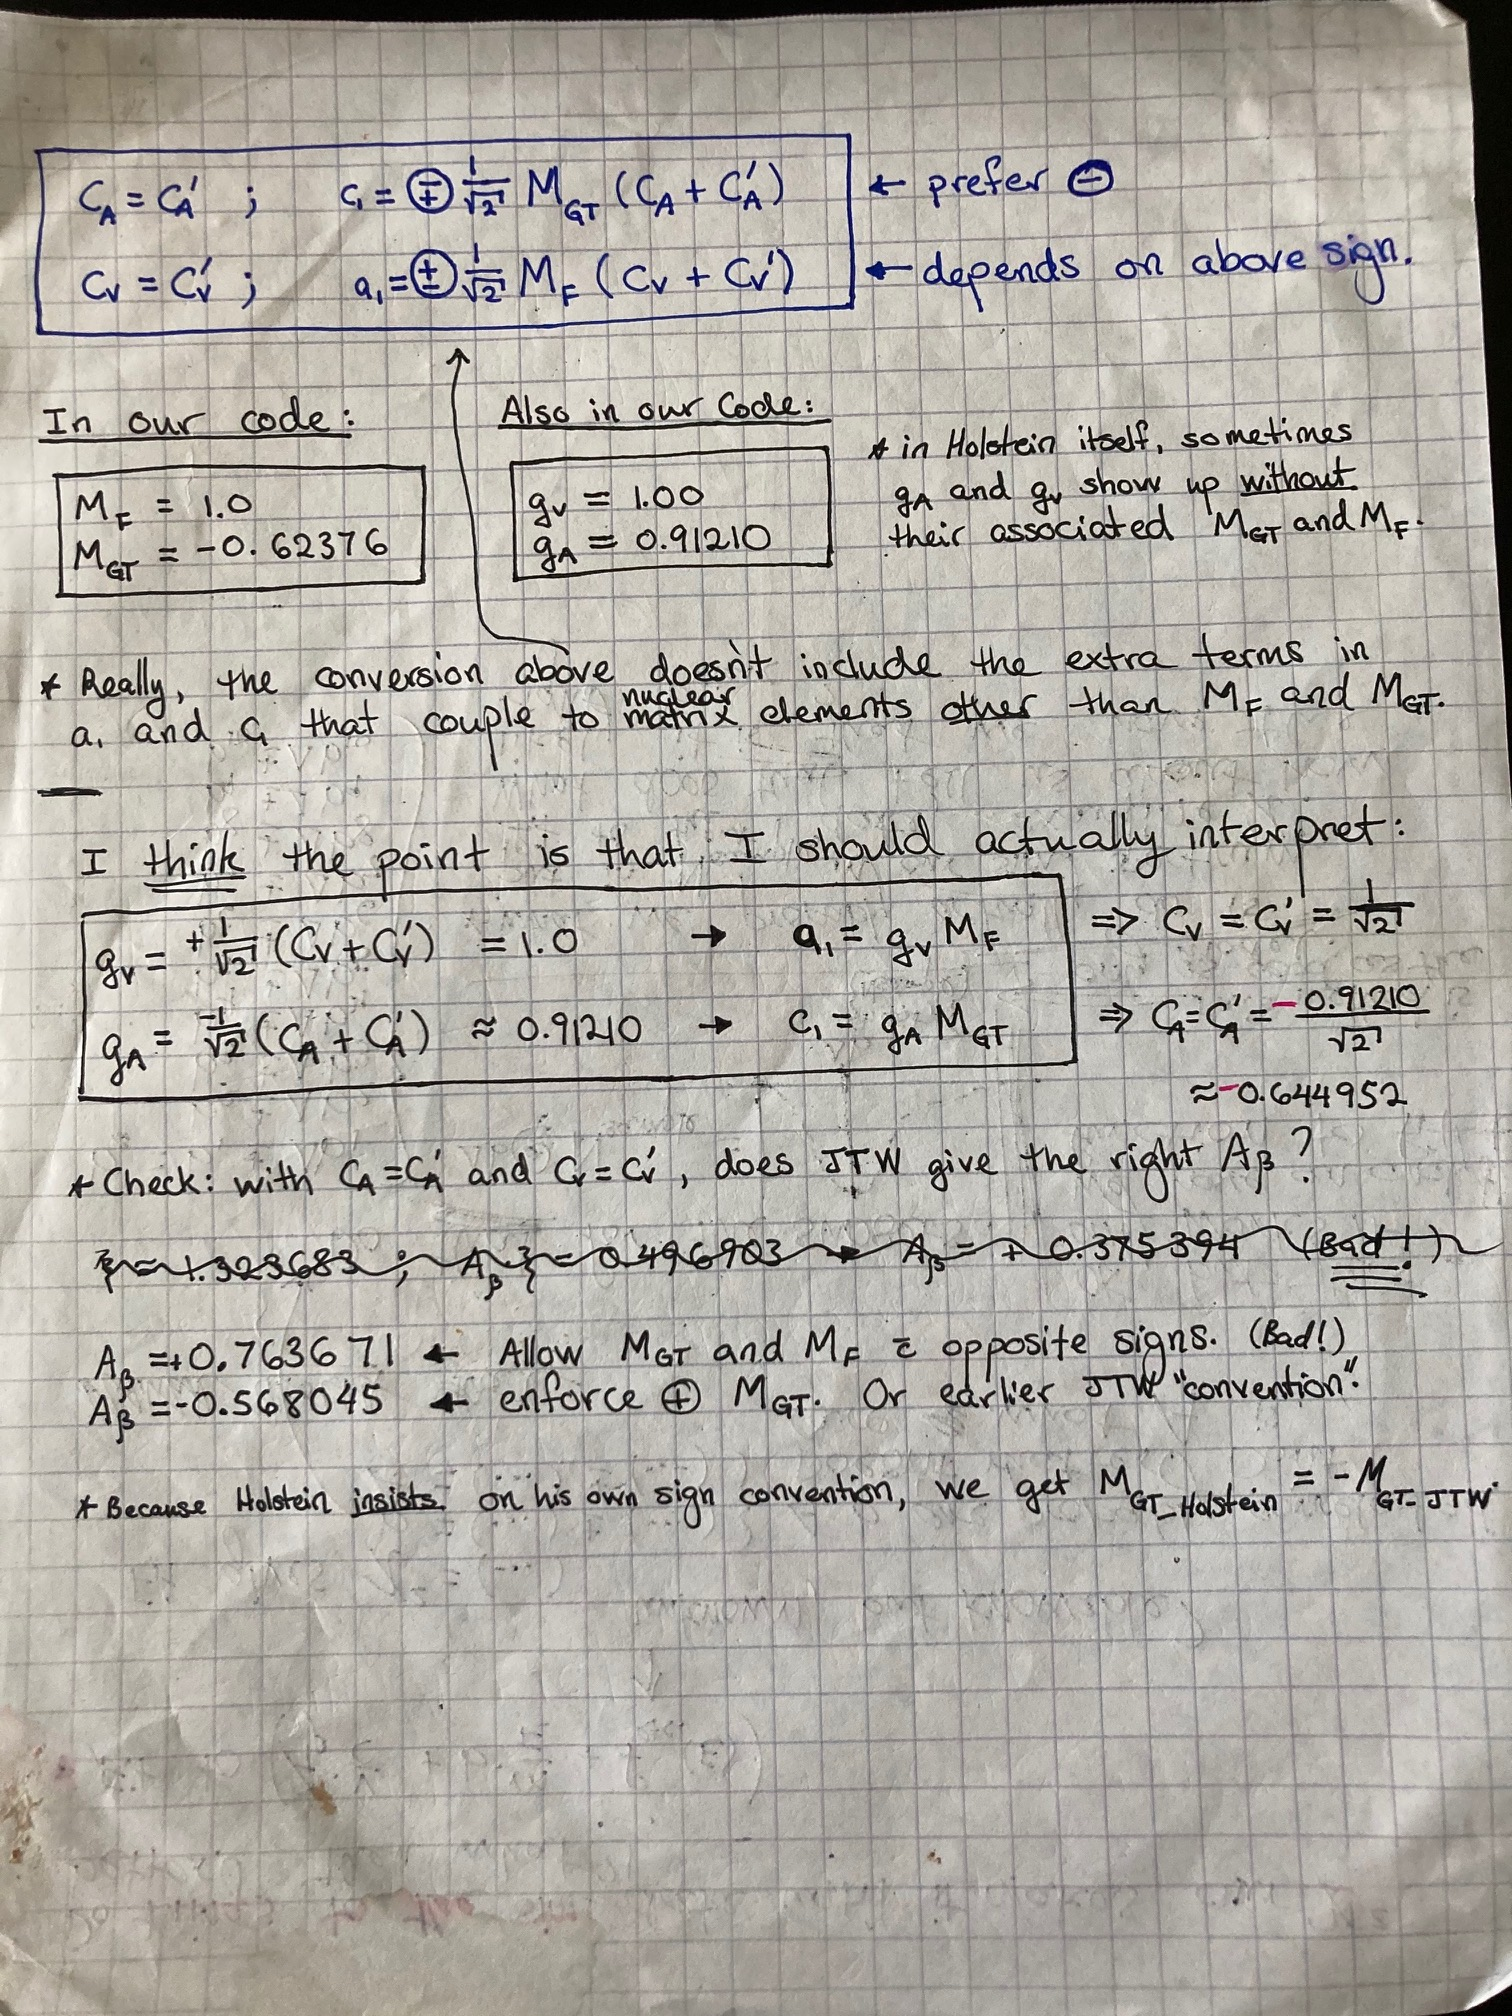
\includegraphics[width=.999\linewidth]
	{Figures/oldnotes_holstein_jtw/image0.jpg} }
	\caption{"Notes 0"}
	\label{fig:notes0}
\end{figure}

\begin{figure}[htb]
	\centering
	{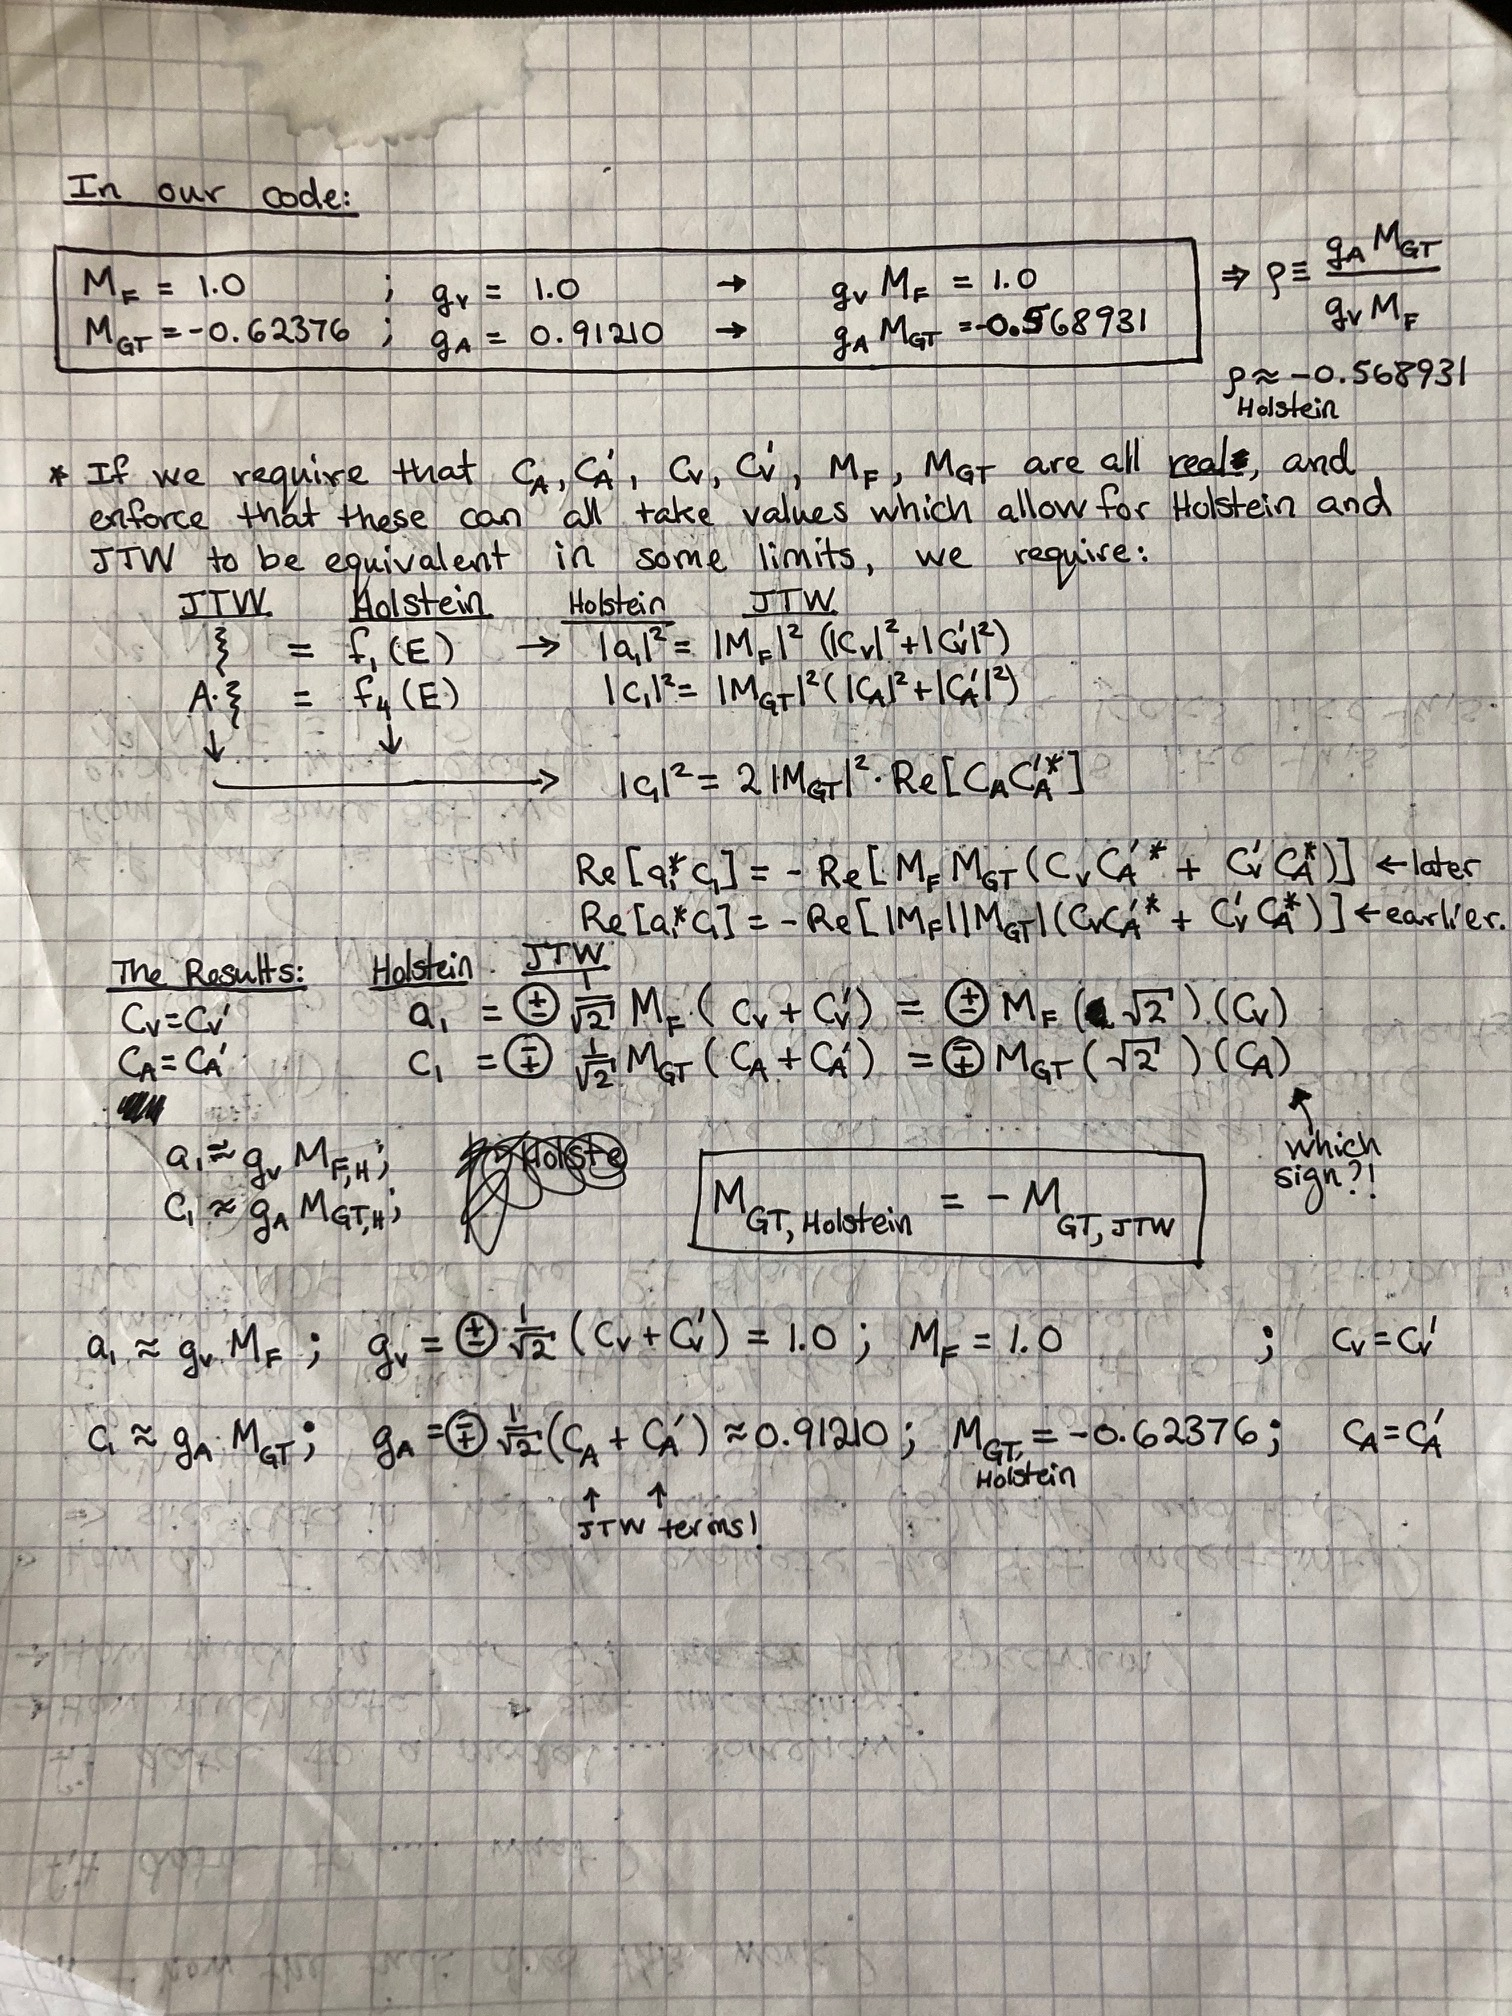
\includegraphics[width=.999\linewidth]
	{Figures/oldnotes_holstein_jtw/image1.jpg} }
	\caption{"Notes 1"}
	\label{fig:notes1}
\end{figure}

\begin{figure}[htb]
	\centering
	{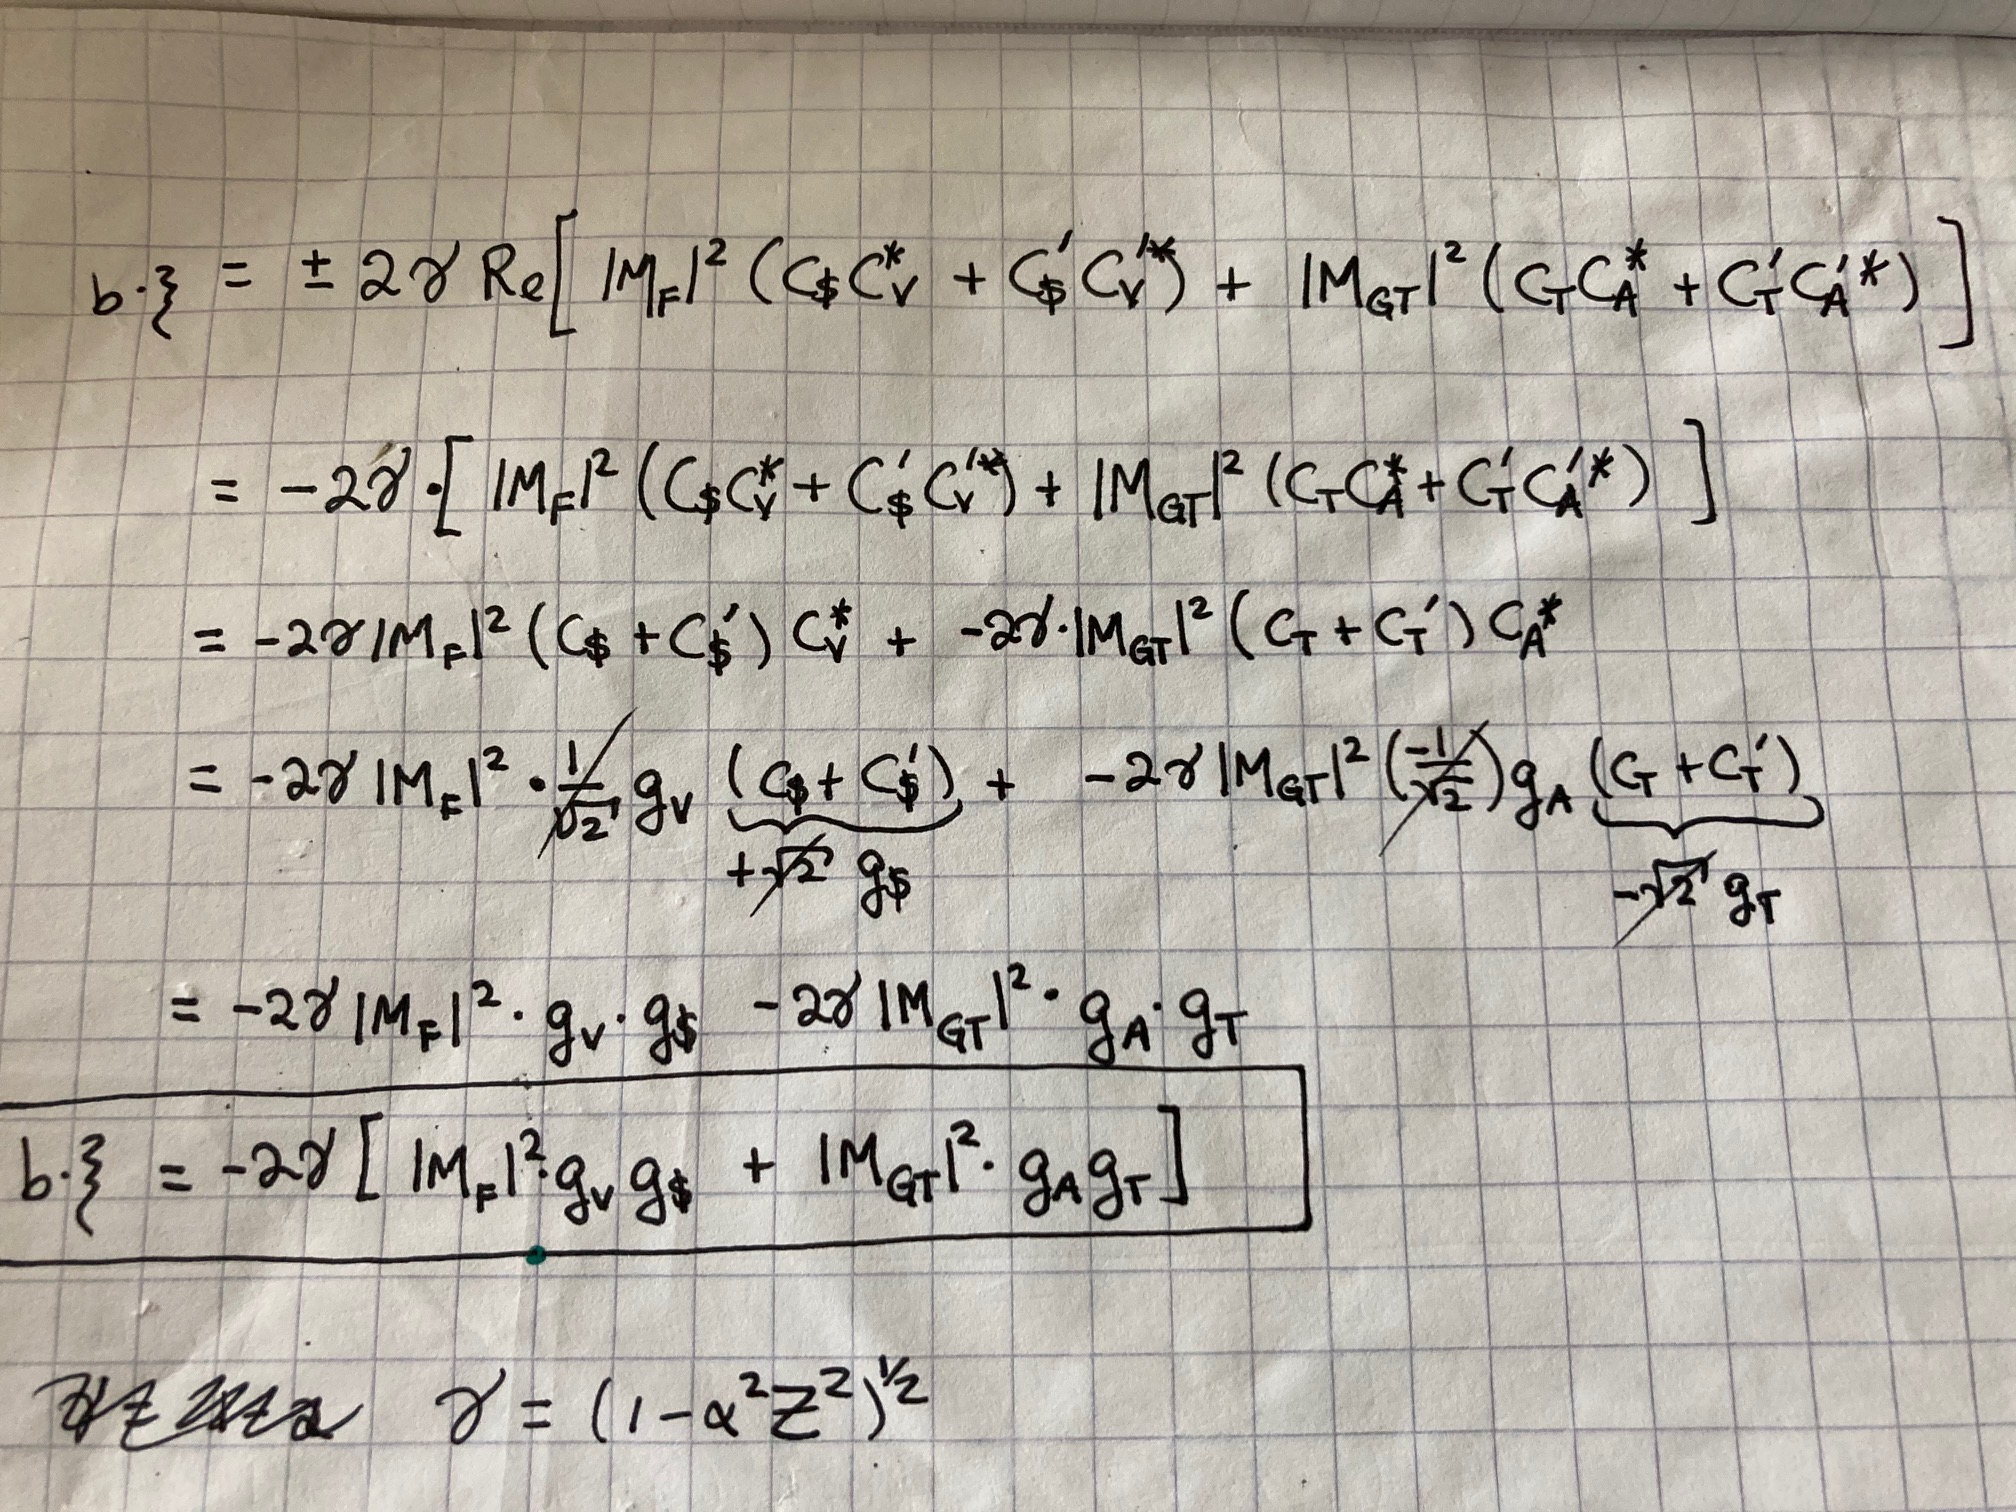
\includegraphics[width=.999\linewidth]
	{Figures/oldnotes_holstein_jtw/image2.jpg} }
	\caption{"Notes 2"}
	\label{fig:notes2}
\end{figure}

\begin{figure}[htb]
	\centering
	{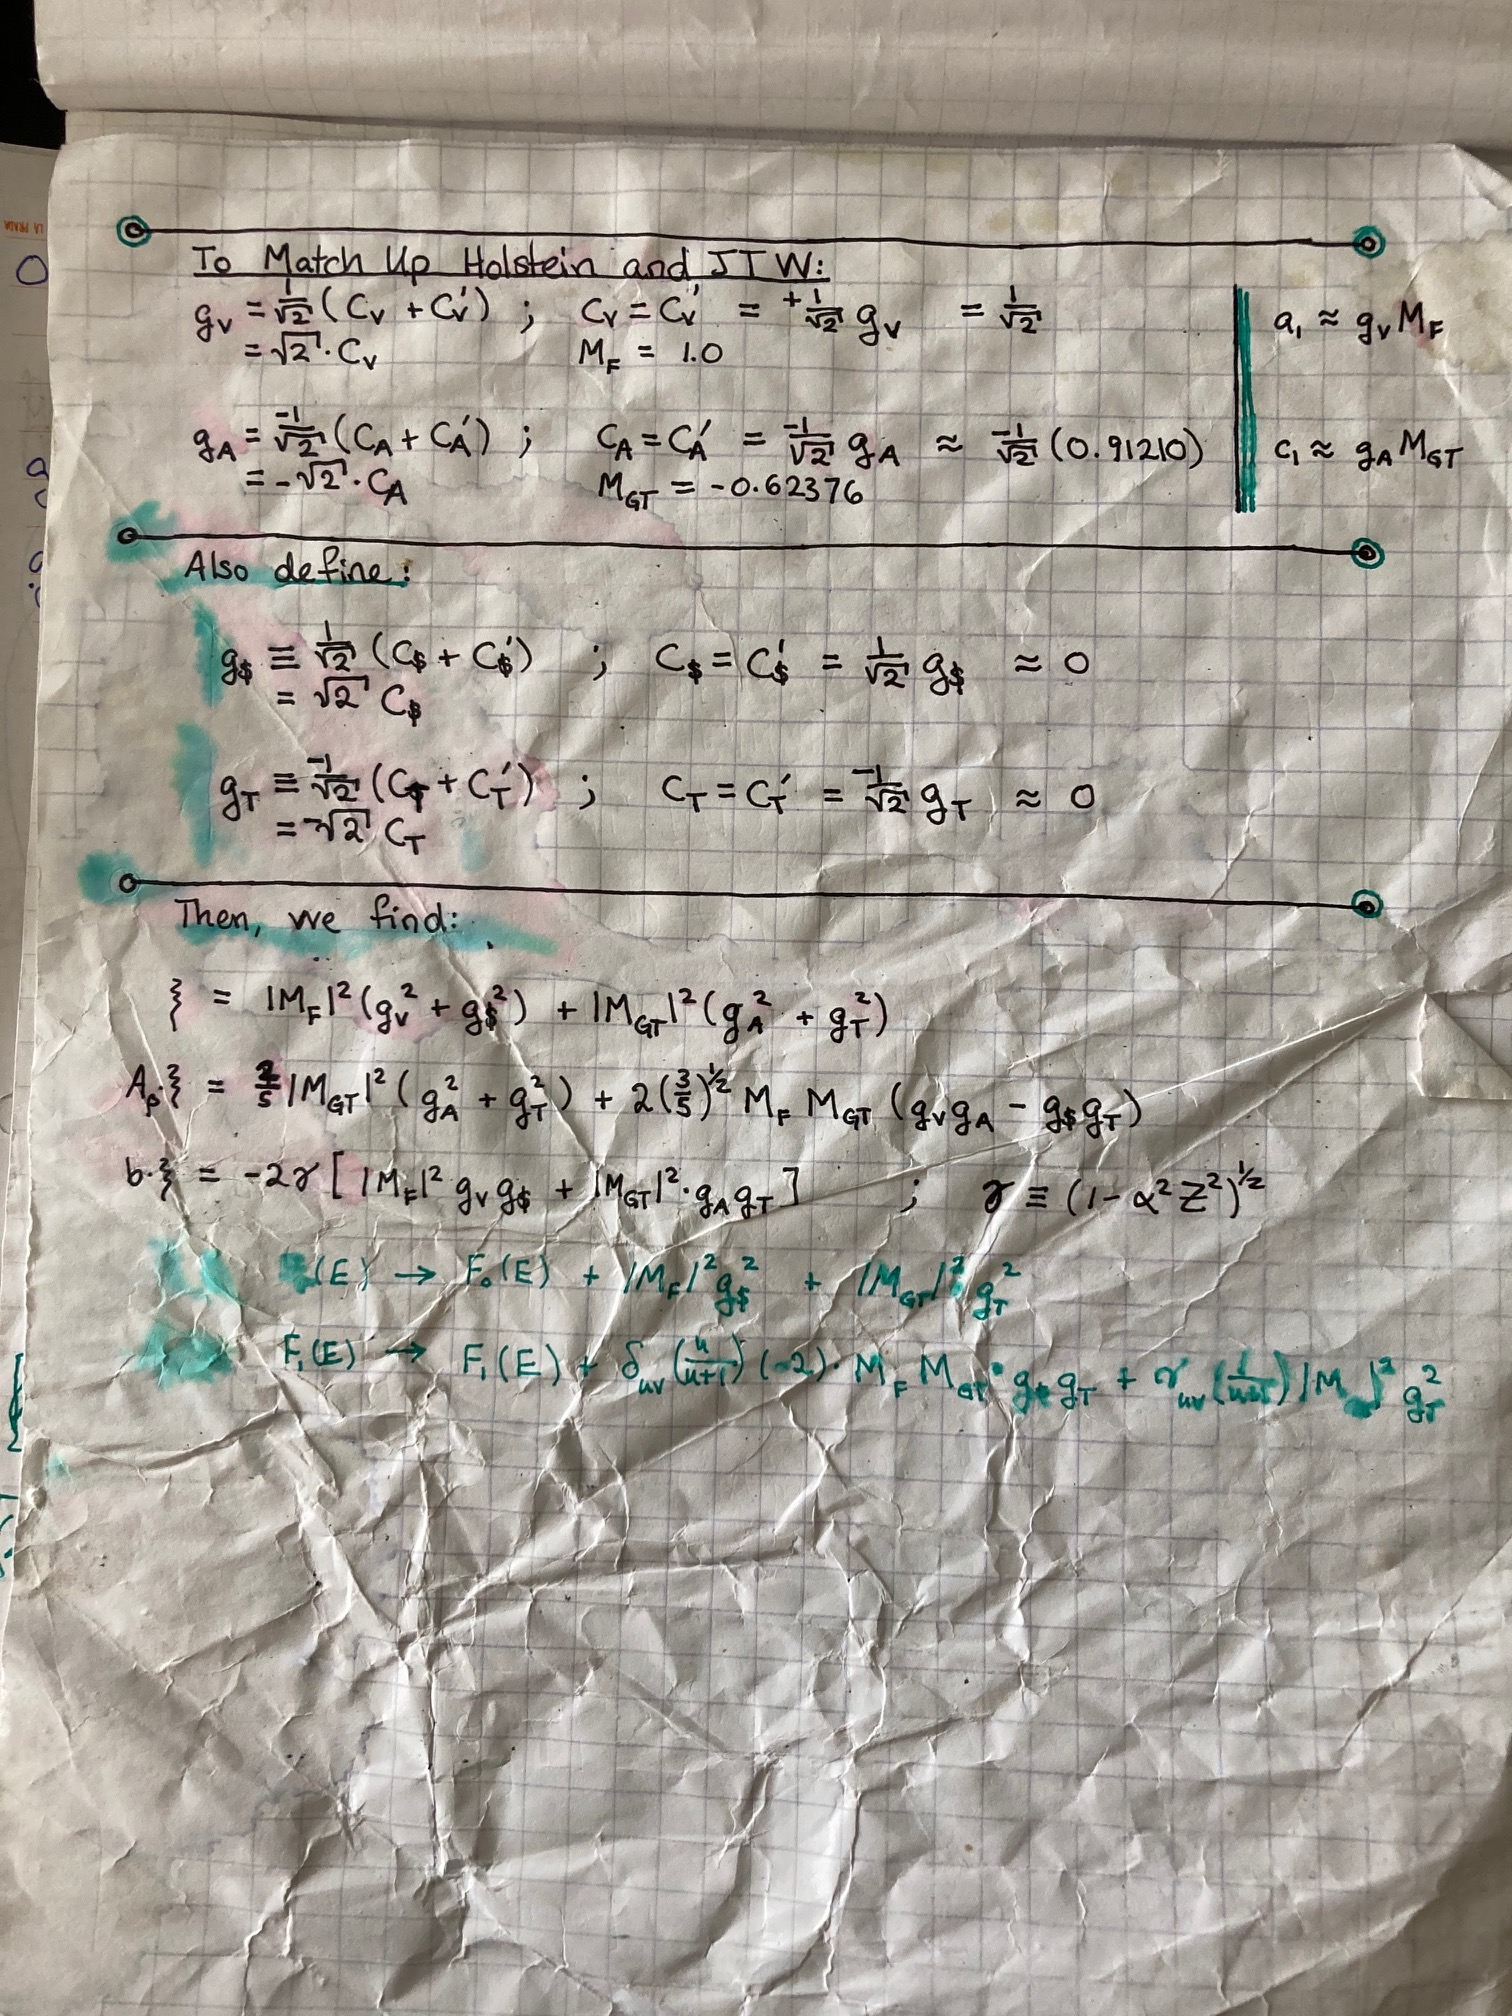
\includegraphics[width=.999\linewidth]
	{Figures/oldnotes_holstein_jtw/image3.jpg} }
	\caption{"Notes 3"}
	\label{fig:notes3}
\end{figure}

\begin{figure}[htb]
	\centering
	{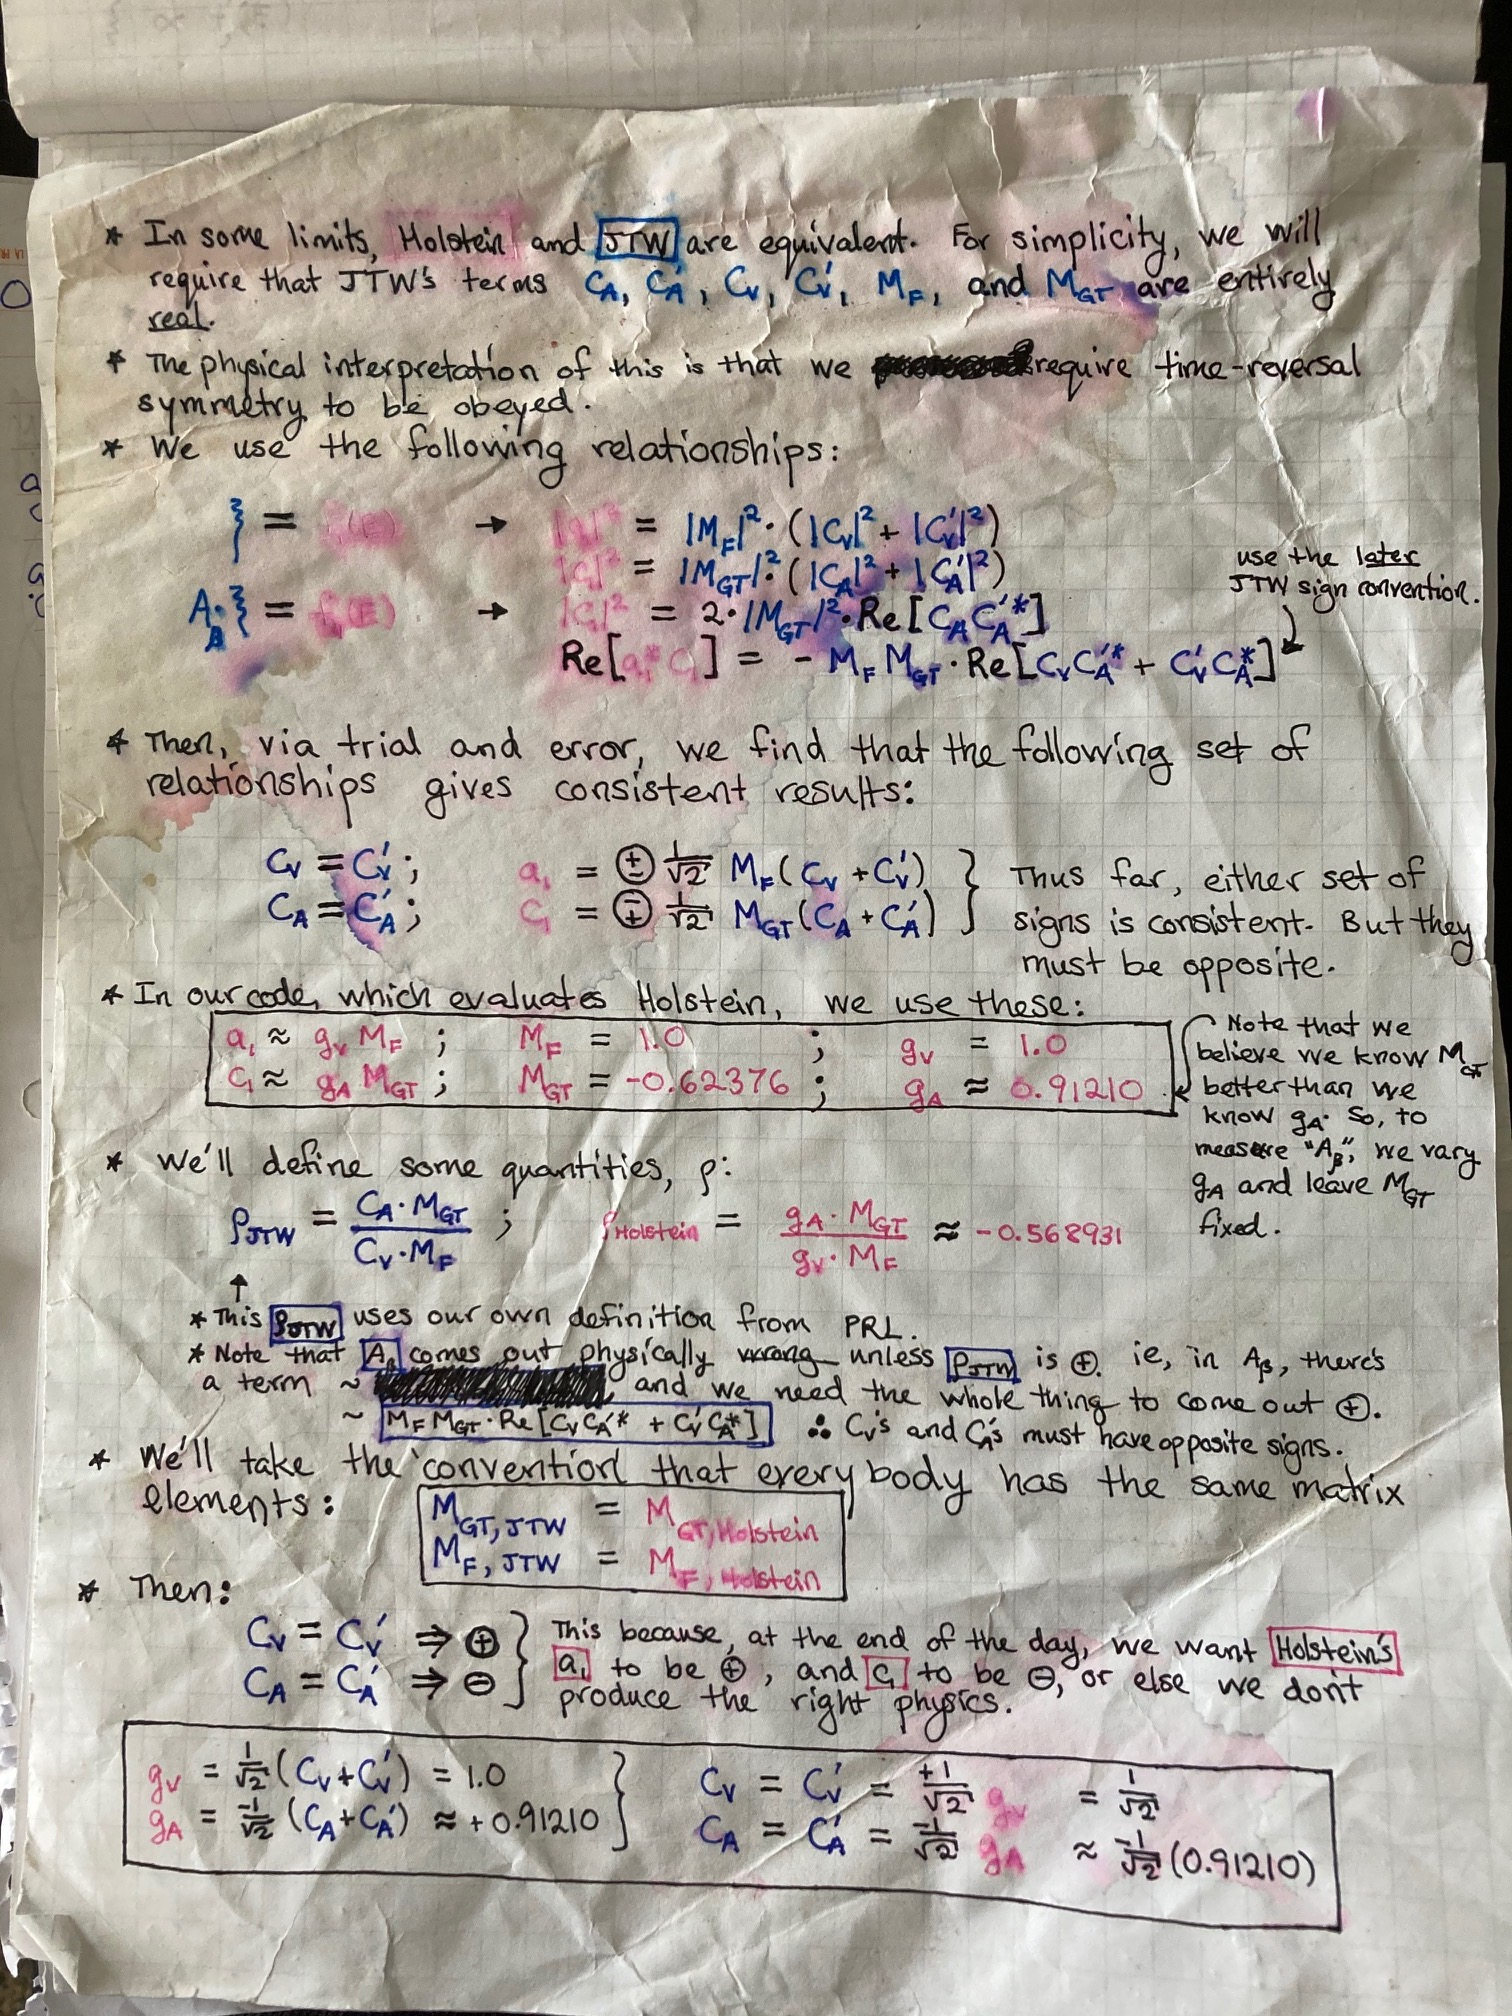
\includegraphics[width=.999\linewidth]
	{Figures/oldnotes_holstein_jtw/image4.jpg} }
	\caption{"Notes 4"}
	\label{fig:notes4}
\end{figure}

\begin{figure}[htb]
	\centering
	{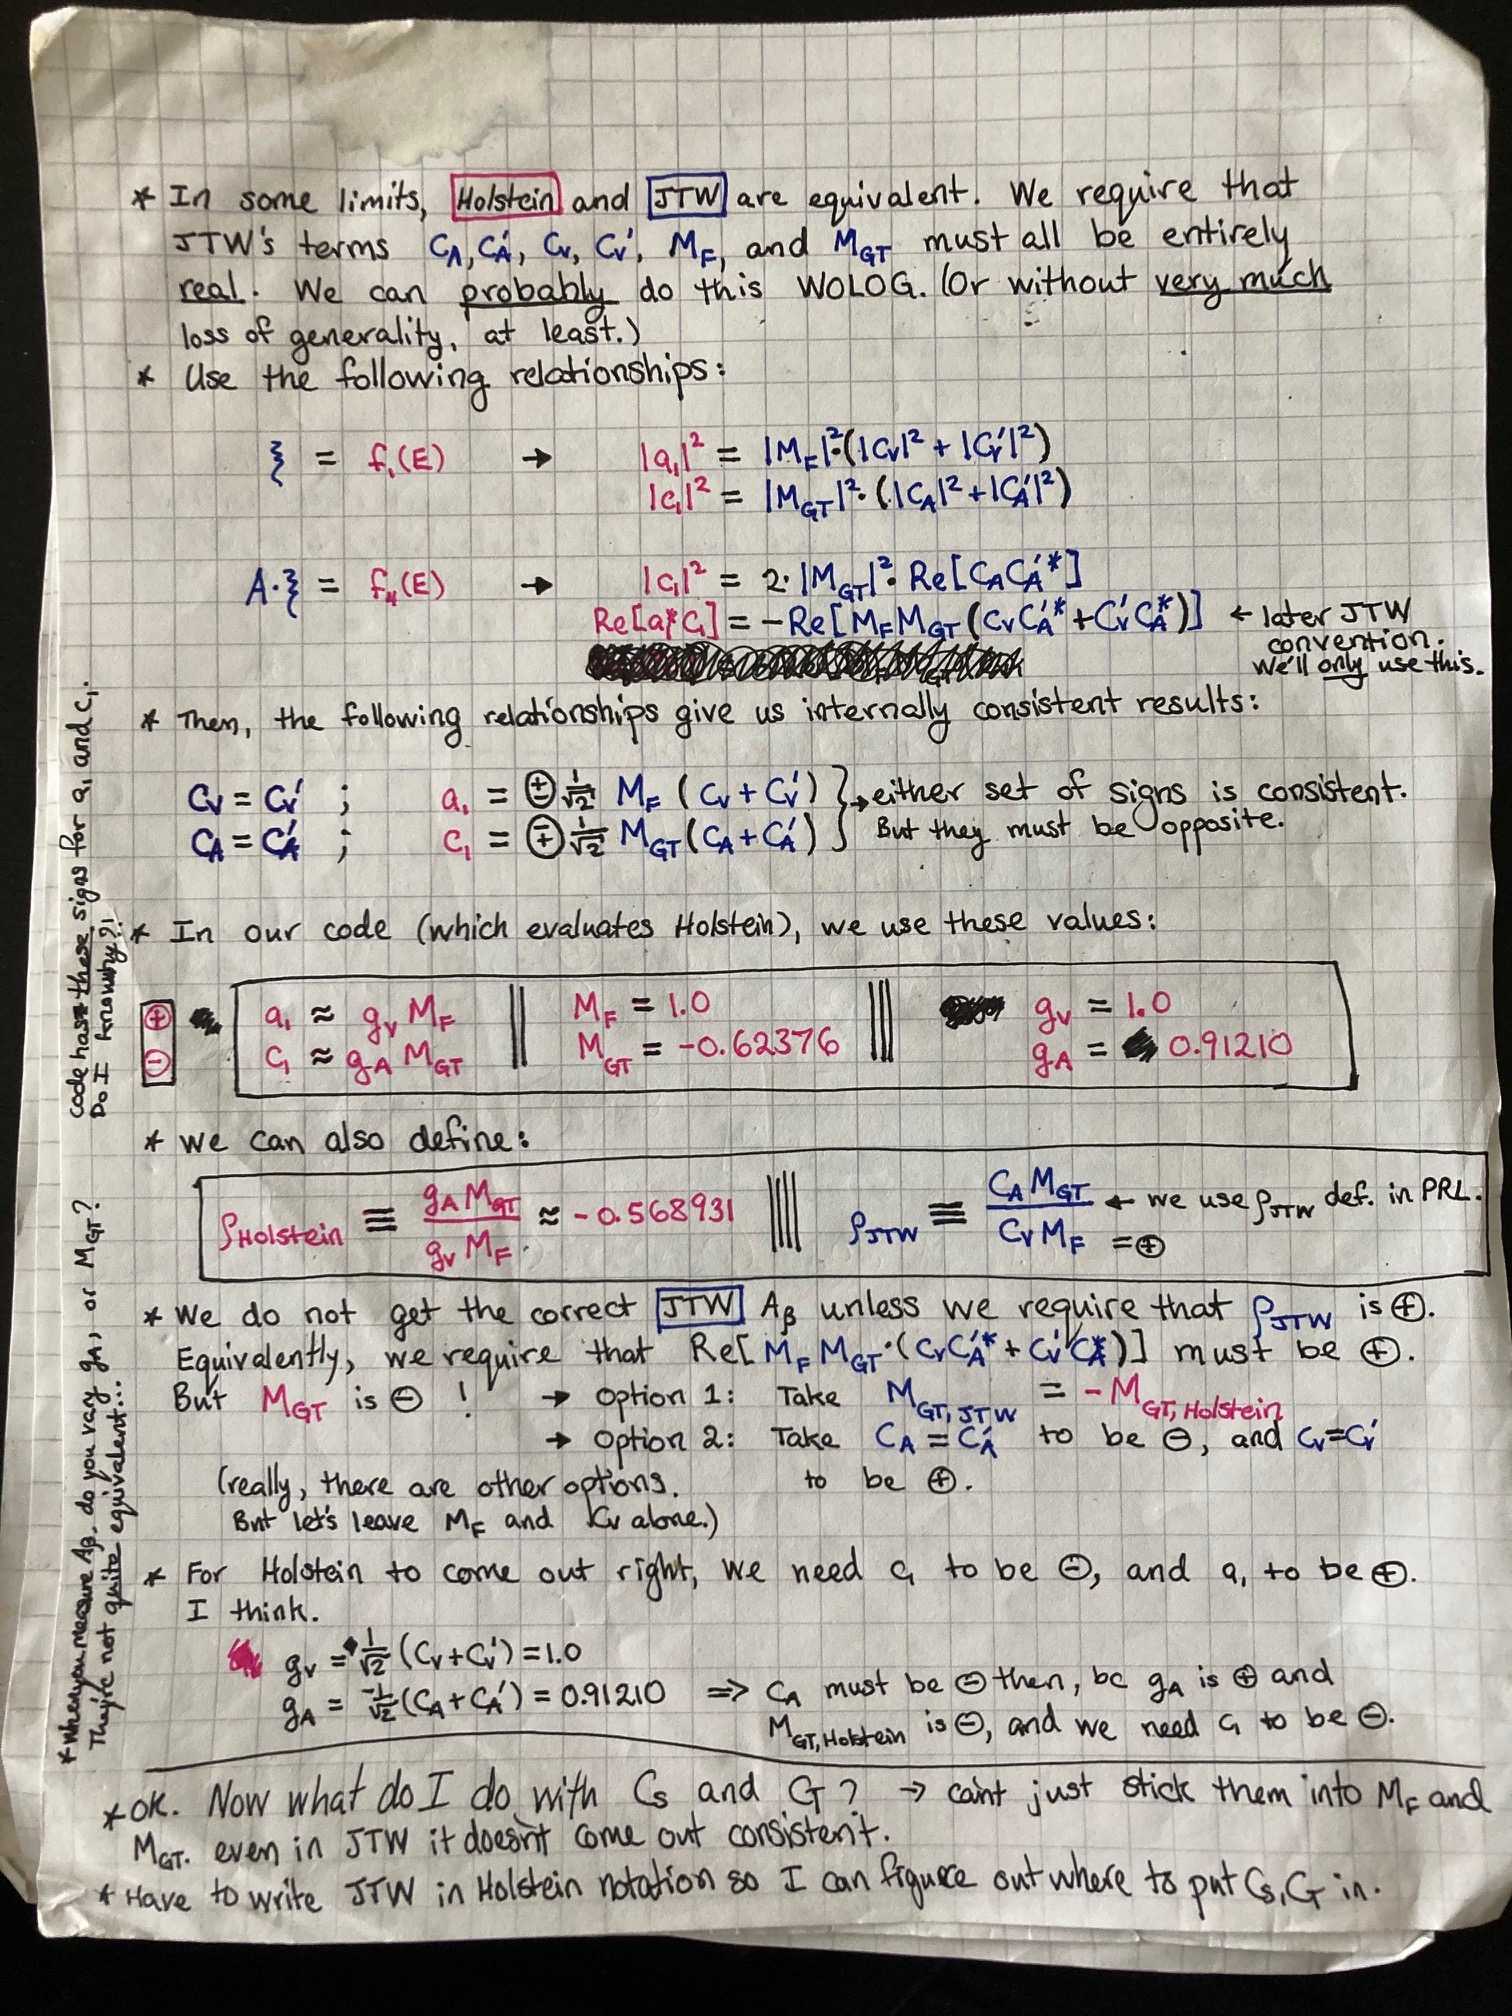
\includegraphics[width=.999\linewidth]
	{Figures/oldnotes_holstein_jtw/image5.jpg} }
	\caption{"Notes 5"}
	\label{fig:notes5}
\end{figure}






